% w nawiasie kwadratowym wpisujemy rodzaj pracy: 
% magisterska, licencjacka, inzynierska
\documentclass[magisterska]{pracadypl}

%% ważne definicje %%
\usepackage{tgtermes}
\usepackage[T1]{fontenc}
\usepackage{polski}
\usepackage[utf8]{inputenc}
\input glyphtounicode
\pdfgentounicode=1
\usepackage{amssymb}
\usepackage{amsmath}
\usepackage{caption}
\usepackage{graphicx}
\setcounter{secnumdepth}{4}  % Ensure subsubsection is numbered
\setcounter{tocdepth}{4}     % Ensure subsubsection appears in TOC
\usepackage{titlesec}
\usepackage{color}
\usepackage{xcolor}
\bibliographystyle{plain}

\def\mgr{magisterska}
\def\lic{licencjacka}
\def\inz{inżynierska}

\def\sk{Słowa kluczowe}
\def\kw{Keywords}
\def\et{Title in English}
%% koniec ważnych definicji %%

%% wypełnia Autor pracy %%

%autor pracy
\author{Gabriel Ozeg}
%numer albumu
\nralbumu{395263}
%tytuł pracy
\title{System antykolizyjny na mikroprocesorze Raspberry Pi}
%kierunek studiów
\kierunek{Informatyka}
%promotor w dopełniaczu
\opiekun{prof. dr hab. Paweł Zajączkowski}
\katedra{Katedra Opiekuna}
%rok
\date{2025}
%Słowa kluczowe:
\slkluczowe{Przetwarzanie obrazu, Głębia obrazu, Metody pomiaru odległości w czasie rzeczywistym, Zastosowania w robotyce}
%tytuł po angielsku
\tytulang{Collision avoidance system on Raspberry Pi microprocessor}
%słowa kluczowe po angielsku
\keywords{Image Processing, Image Depth, Real-Time Distance Measurement Methods, Applications in Robotics}
%% koniec ważnych definicji %%

%% APD %%
%% w systemie APD należy jeszcze wpisać, poza powyższymi informacjami, streszczenie oraz streszczenie w języku angielskim  %%


%%% definicje %%%
\def\pd{\noindent \textbf{Dowód.~}} %%początek dowodu
\def\kd{\hfill\mbox{$\rule{2mm}{2mm}$}} %%koniec dowodu
\newtheorem{defi}{Definicja}[section]
\newtheorem{uwaga}{Uwaga}[section]
\newtheorem{tw}{Twierdzenie}[section]
\newtheorem{lem}{Lemat}[section]
\newtheorem{wn}{Wniosek}[section]
\renewcommand\thetw{\thesection.\arabic{tw}.}
\renewcommand\thedefi{\thesection.\arabic{defi}.}
\renewcommand\theuwaga{\thesection.\arabic{uwaga}.}
\renewcommand\thetw{\thesection.\arabic{tw}.}
\renewcommand\thelem{\thesection.\arabic{lem}.}
\renewcommand\thewn{\thesection.\arabic{wn}.}
%
\definecolor{wmiigreen}{rgb}{0.0, 0.5, 0.0}
\titleformat{\chapter}[display]
  {\normalfont\huge\bfseries\color{wmiigreen}}{\chaptertitlename\ \thechapter}{10pt}{\Huge}
 %
\linespread{1.3}
%%% koniec definicji %%%


\begin{document}

\maketitle
\tableofcontents
\newpage



\chapter{Wstęp}

We wstępie pracy dyplomowej powinien znaleźć się opis wkładu własnego studenta w uzyskanie przedstawianych wyników a także informacje o podstawowych źródłach, na podstawie których student przygotował pracę.


\chapter{Podstawowe pojęcia}

  \section{Definicje i własności}

  W niniejszej części pracy podane zostaną pojęcia niezbędne w późniejszych rozważaniach (patrz \cite{Kostrykin} lub \cite{Lang}).
  \begin{defi}
  Niech $G$ będzie niepustym zbiorem. Działaniem w $G$ nazywamy dowolne odwzorowanie $\circ:G\times G\to G$.
  \end{defi}

  \begin{defi}
  Niech $G$ będzie niepustym zbiorem, $\circ$ działaniem w $G$. Element $e\in G$ nazywamy neutralnym (działania $\circ$), jeśli dla każdego $a\in G$ mamy $a\circ e=e\circ a=a$.
  \end{defi}

  \begin{lem}\label{lem:element_neutralny}
  Jeśli działanie $\circ$ w $G$ posiada element neutralny, to jest on jeden.
  \end{lem}
  \pd Niech $e,e'\in G$ będą dwoma elementami neutralnymi. Wtedy
  \begin{equation}\label{eq:element_neutralny}
  e=e'\circ e=e'.
  \end{equation}
  Zatem element neutralny jest jeden. \kd


  \section{Przykłady}

  Działaniem w zbiorze liczb naturalnych jest dodawanie, natomiast działaniem w tym zbiorze nie jest odejmowanie.


\chapter{Część główna}

\section{Przetwarzanie obrazu}

Przetwarzanie obrazu to dziedzina informatyki i inżynierii zajmująca się analizą, modyfikacją i interpretacją obrazów cyfrowych za pomocą metod numerycznych i algorytmów komputerowych. Jej celem jest poprawa jakości obrazów, ekstrakcja informacji, segmentacja obiektów lub ich klasyfikacja. Przetwarzanie obrazu znajduje zastosowanie w wielu obszarach, takich jak medycyna (np. analiza zdjęć RTG), przemysł (np. kontrola jakości), bezpieczeństwo (np. rozpoznawanie twarzy), robotyka oraz systemy wizyjne pojazdów autonomicznych. Dzięki połączeniu technik matematycznych, statystycznych i sztucznej inteligencji możliwe jest coraz bardziej precyzyjne i automatyczne rozumienie zawartości obrazów.

\subsection{Rodzaje kamer i techniki używane do estymacji głębi}

\subsubsection{Monocular Vision}

\begin{figure}[h]  % 'h' means "here", it places the figure at the current location in the document
    \centering  % Centers the image
    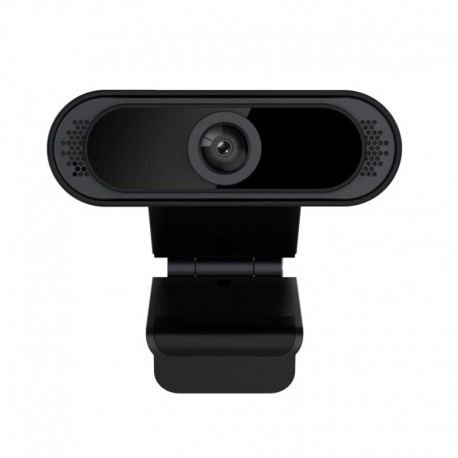
\includegraphics[width=0.3\textwidth]{images/MONO.jpg}  % Adjust the path and width as necessary
    \captionsetup{labelformat=empty, font=footnotesize}
    \caption{Źródło: https://cell-kom.com/inne/21454-kamera-internetowa-full-hd-b16-1080p-5900217390350.html}
    \label{fig:mono}  % Optional: use to refer to this image later in the text
\end{figure}


Monocular vision (widzenie monokularne) to technika pozyskiwania informacji wizualnych przy użyciu tylko jednejkamery, czyli takiej, która rejestruje obraz z pojedynczego punktu widzenia — podobnie jak jedno oko u człowieka.\\

\begin{minipage}[t]{0.45\textwidth}
\textbf{Zalety:}
\begin{itemize}
  \item Niska cena: Wymaga tylko jednej kamery – tańsze niż systemy stereo lub LiDAR.

  \item Mniejsze zużycie energii: Idealne dla urządzeń mobilnych, dronów, robotów.

  \item Prosta instalacja: Nie trzeba kalibrować dwóch kamer ani martwić się synchronizacją.

  \item Łatwo dostępne dane: Każdy smartfon lub laptop może być źródłem obrazu.

  \item Możliwość działania w czasie rzeczywistym: Przy odpowiedniej optymalizacji algorytmu.
\end{itemize}
\end{minipage}
\hfill
\begin{minipage}[t]{0.45\textwidth}
\textbf{Wady:}
\begin{itemize}
  \item Brak skali bezwzględnej: Nie wiadomo, czy obiekt jest 1 metr czy 10 metrów od kamery bez dodatkowej informacji (np. IMU, GPS).

  \item Słabsza dokładność głębokości: W porównaniu do stereowizji lub sensorów ToF/LiDAR.

  \item Trudności w scenach jednorodnych: Powtarzalne tekstury lub słabe oświetlenie utrudniają analizę.

  \item Potrzeba ruchu kamery (np. w SLAM): Dla bardziej precyzyjnej rekonstrukcji sceny.
\end{itemize}
\end{minipage}

\subsubsection{Stereo Vision}

\begin{figure}[h]  % 'h' means "here", it places the figure at the current location in the document
    \centering  % Centers the image
    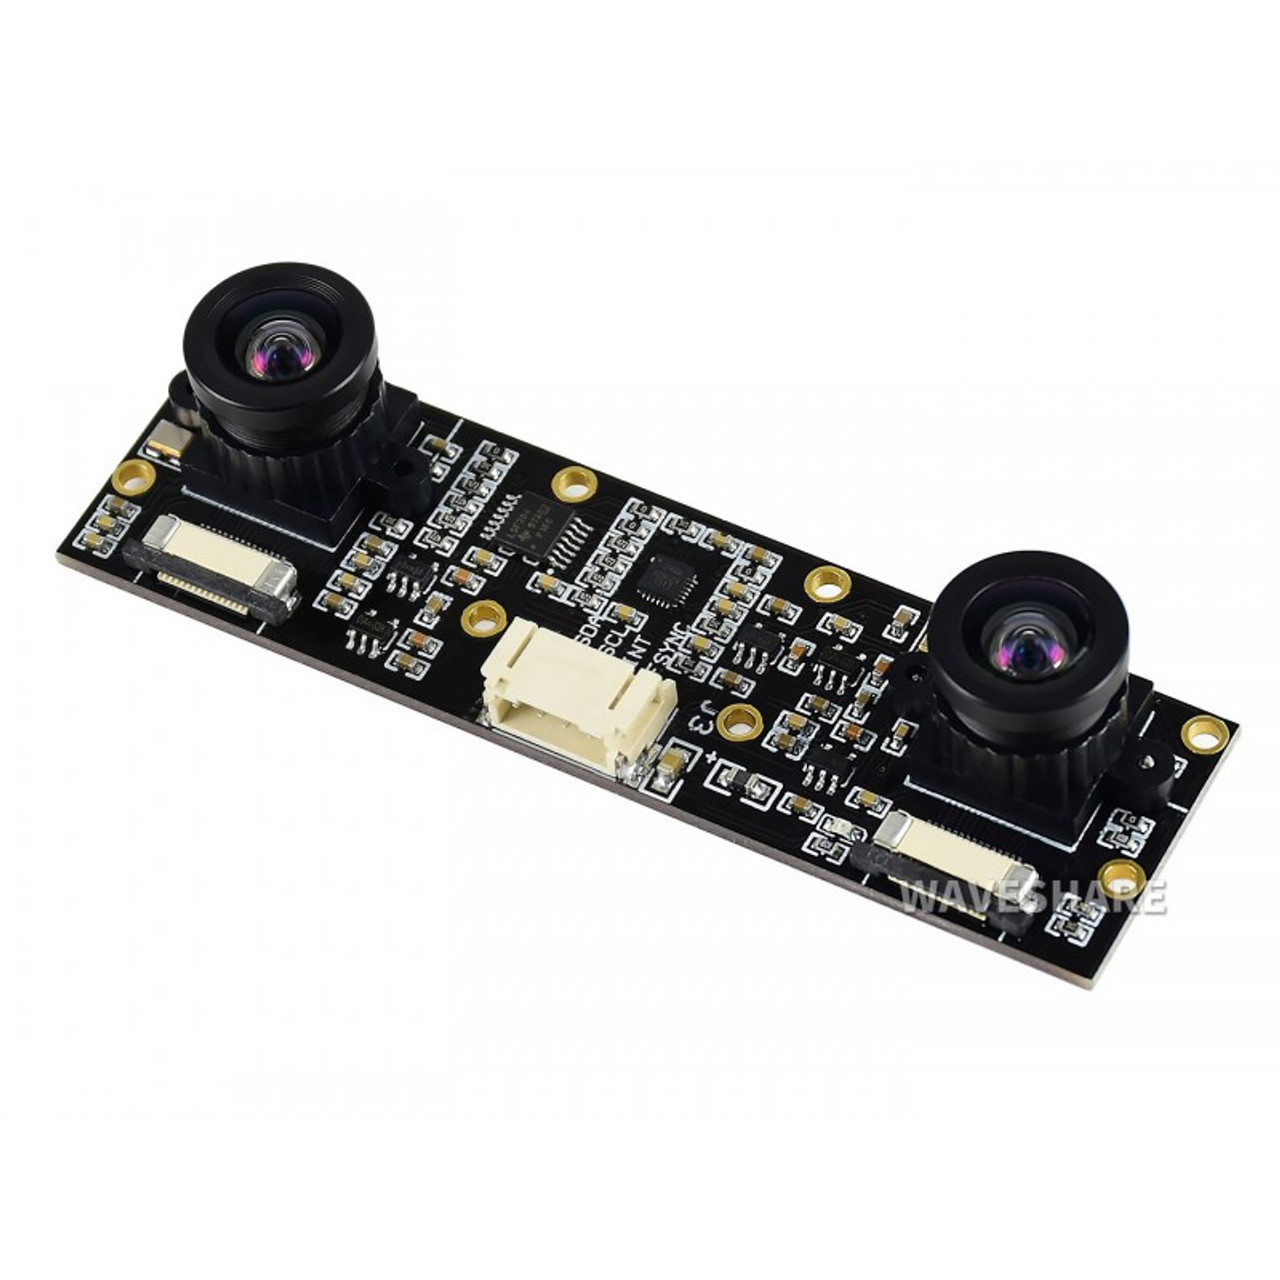
\includegraphics[width=0.5\textwidth]{images/STEREO.jpg}  % Adjust the path and width as necessary
    \captionsetup{labelformat=empty, font=footnotesize}
    \caption{Źródło: https://cell-kom.com/inne/21454-kamera-internetowa-full-hd-b16-1080p-5900217390350.html}
    \label{fig:mono}  % Optional: use to refer to this image later in the text
\end{figure}

Stereo vision (widzenie stereoskopowe) to technika komputerowego przetwarzania obrazu, która umożliwia określenie głębokości i kształtu obiektów w scenie poprzez analizę dwóch obrazów zarejestrowanych przez dwie kamery umieszczone w pewnej odległości od siebie (zwykle poziomej — jak oczy u człowieka).

Porównując różnice (czyli dysparycje) w położeniu tych samych punktów na lewym i prawym obrazie, można obliczyć odległość obiektów od kamer — dzięki znanym wzorom geometrycznym (triangulacja).


\begin{minipage}[t]{0.45\textwidth}
\textbf{Zalety:}
\begin{itemize}
  \item Prawdziwa głębokość geometryczna — możliwa do przeliczenia na metry.

  \item Działa w czasie rzeczywistym — przy użyciu odpowiedniego sprzętu (np. ZED Camera, Intel RealSense).

  \item Nie wymaga poruszania kamerą — wystarczą dwa obrazy z dwóch stałych punktów.

  \item Nadaje się do zastosowań mobilnych i przemysłowych (robotyka, autonomiczne pojazdy, pomiary 3D).
\end{itemize}
\end{minipage}
\hfill
\begin{minipage}[t]{0.45\textwidth}
\textbf{Wady:}
\begin{itemize}
  \item Wrażliwość na warunki oświetleniowe — słabe światło, odbicia lub brak tekstury mogą uniemożliwić porównanie obrazów.

  \item Potrzebna kalibracja — kamery muszą być dokładnie skalibrowane (ustalenie ich pozycji i parametrów).

  \item Złożoność obliczeniowa — dopasowanie punktów między obrazami może być kosztowne.

  \item Martwe strefy — obiekty o jednolitej teksturze (np. ściana) mogą nie dawać użytecznych danych.
\end{itemize}
\end{minipage}

\subsubsection{Structure from Motion (SfM)}

\begin{figure}[h]  % 'h' means "here", it places the figure at the current location in the document
    \centering  % Centers the image
    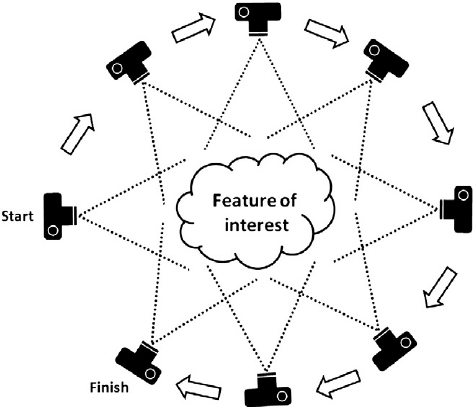
\includegraphics[width=0.5\textwidth]{images/SFM.png}  % Adjust the path and width as necessary
    \captionsetup{labelformat=empty, font=footnotesize}
    \caption{Źródło: https://cell-kom.com/inne/21454-kamera-internetowa-full-hd-b16-1080p-5900217390350.html}
    \label{fig:mono}  % Optional: use to refer to this image later in the text
\end{figure}

Structure from Motion (SfM) to technika wizyjna, która pozwala zrekonstruować strukturę trójwymiarową sceny oraz trajektorię ruchu kamery na podstawie zwykłych zdjęć lub klatek wideo wykonanych jedną lub wieloma kamerami, które poruszają się względem sceny.

SfM działa tak:
Wykrywa punkty charakterystyczne (np. rogi, krawędzie) na zdjęciach.
Śledzi ich pozycje na kolejnych ujęciach.
Oblicza względne pozycje kamer i 3D współrzędne punktów w scenie – czyli rekonstruuje kształt i ruch.

\begin{minipage}[t]{0.45\textwidth}
\textbf{Zalety:}
\begin{itemize}
  \item Umożliwia 3D rekonstrukcję z pojedynczej kamery – wystarczy poruszać kamerą wokół obiektu.

  \item Niski koszt sprzętowy – można wykorzystać zwykły aparat lub smartfon.

  \item Brak potrzeby kalibracji sprzętu z góry – SfM może działać nawet na niekalibrowanych zdjęciach.

  \item Wysoka dokładność w scenach z dobrą teksturą.

  \item Zastosowania w wielu dziedzinach: archeologia, kartografia, VR, robotyka, fotogrametria.
\end{itemize}
\end{minipage}
\hfill
\begin{minipage}[t]{0.45\textwidth}
\textbf{Wady:}
\begin{itemize}
  \item Wymaga wielu zdjęć z różnych perspektyw – nie działa dobrze, jeśli kamera stoi w miejscu.

  \item Problemy w scenach z małą teksturą – np. gładkie ściany, powierzchnie bez szczegółów.

  \item Czasochłonność obliczeniowa – rekonstrukcja może trwać długo, szczególnie dla dużych zbiorów zdjęć.

  \item Brak skali bezwzględnej – SfM daje model „w skali względnej”, czyli np. 1 m może być 1 cm, jeśli nie ma referencji.

  \item Wrażliwe na rozmycie, szum, ruch obiektów w tle.
\end{itemize}
\end{minipage}

\subsubsection{Time-of-Flight (ToF)}

\begin{figure}[h]  % 'h' means "here", it places the figure at the current location in the document
    \centering  % Centers the image
    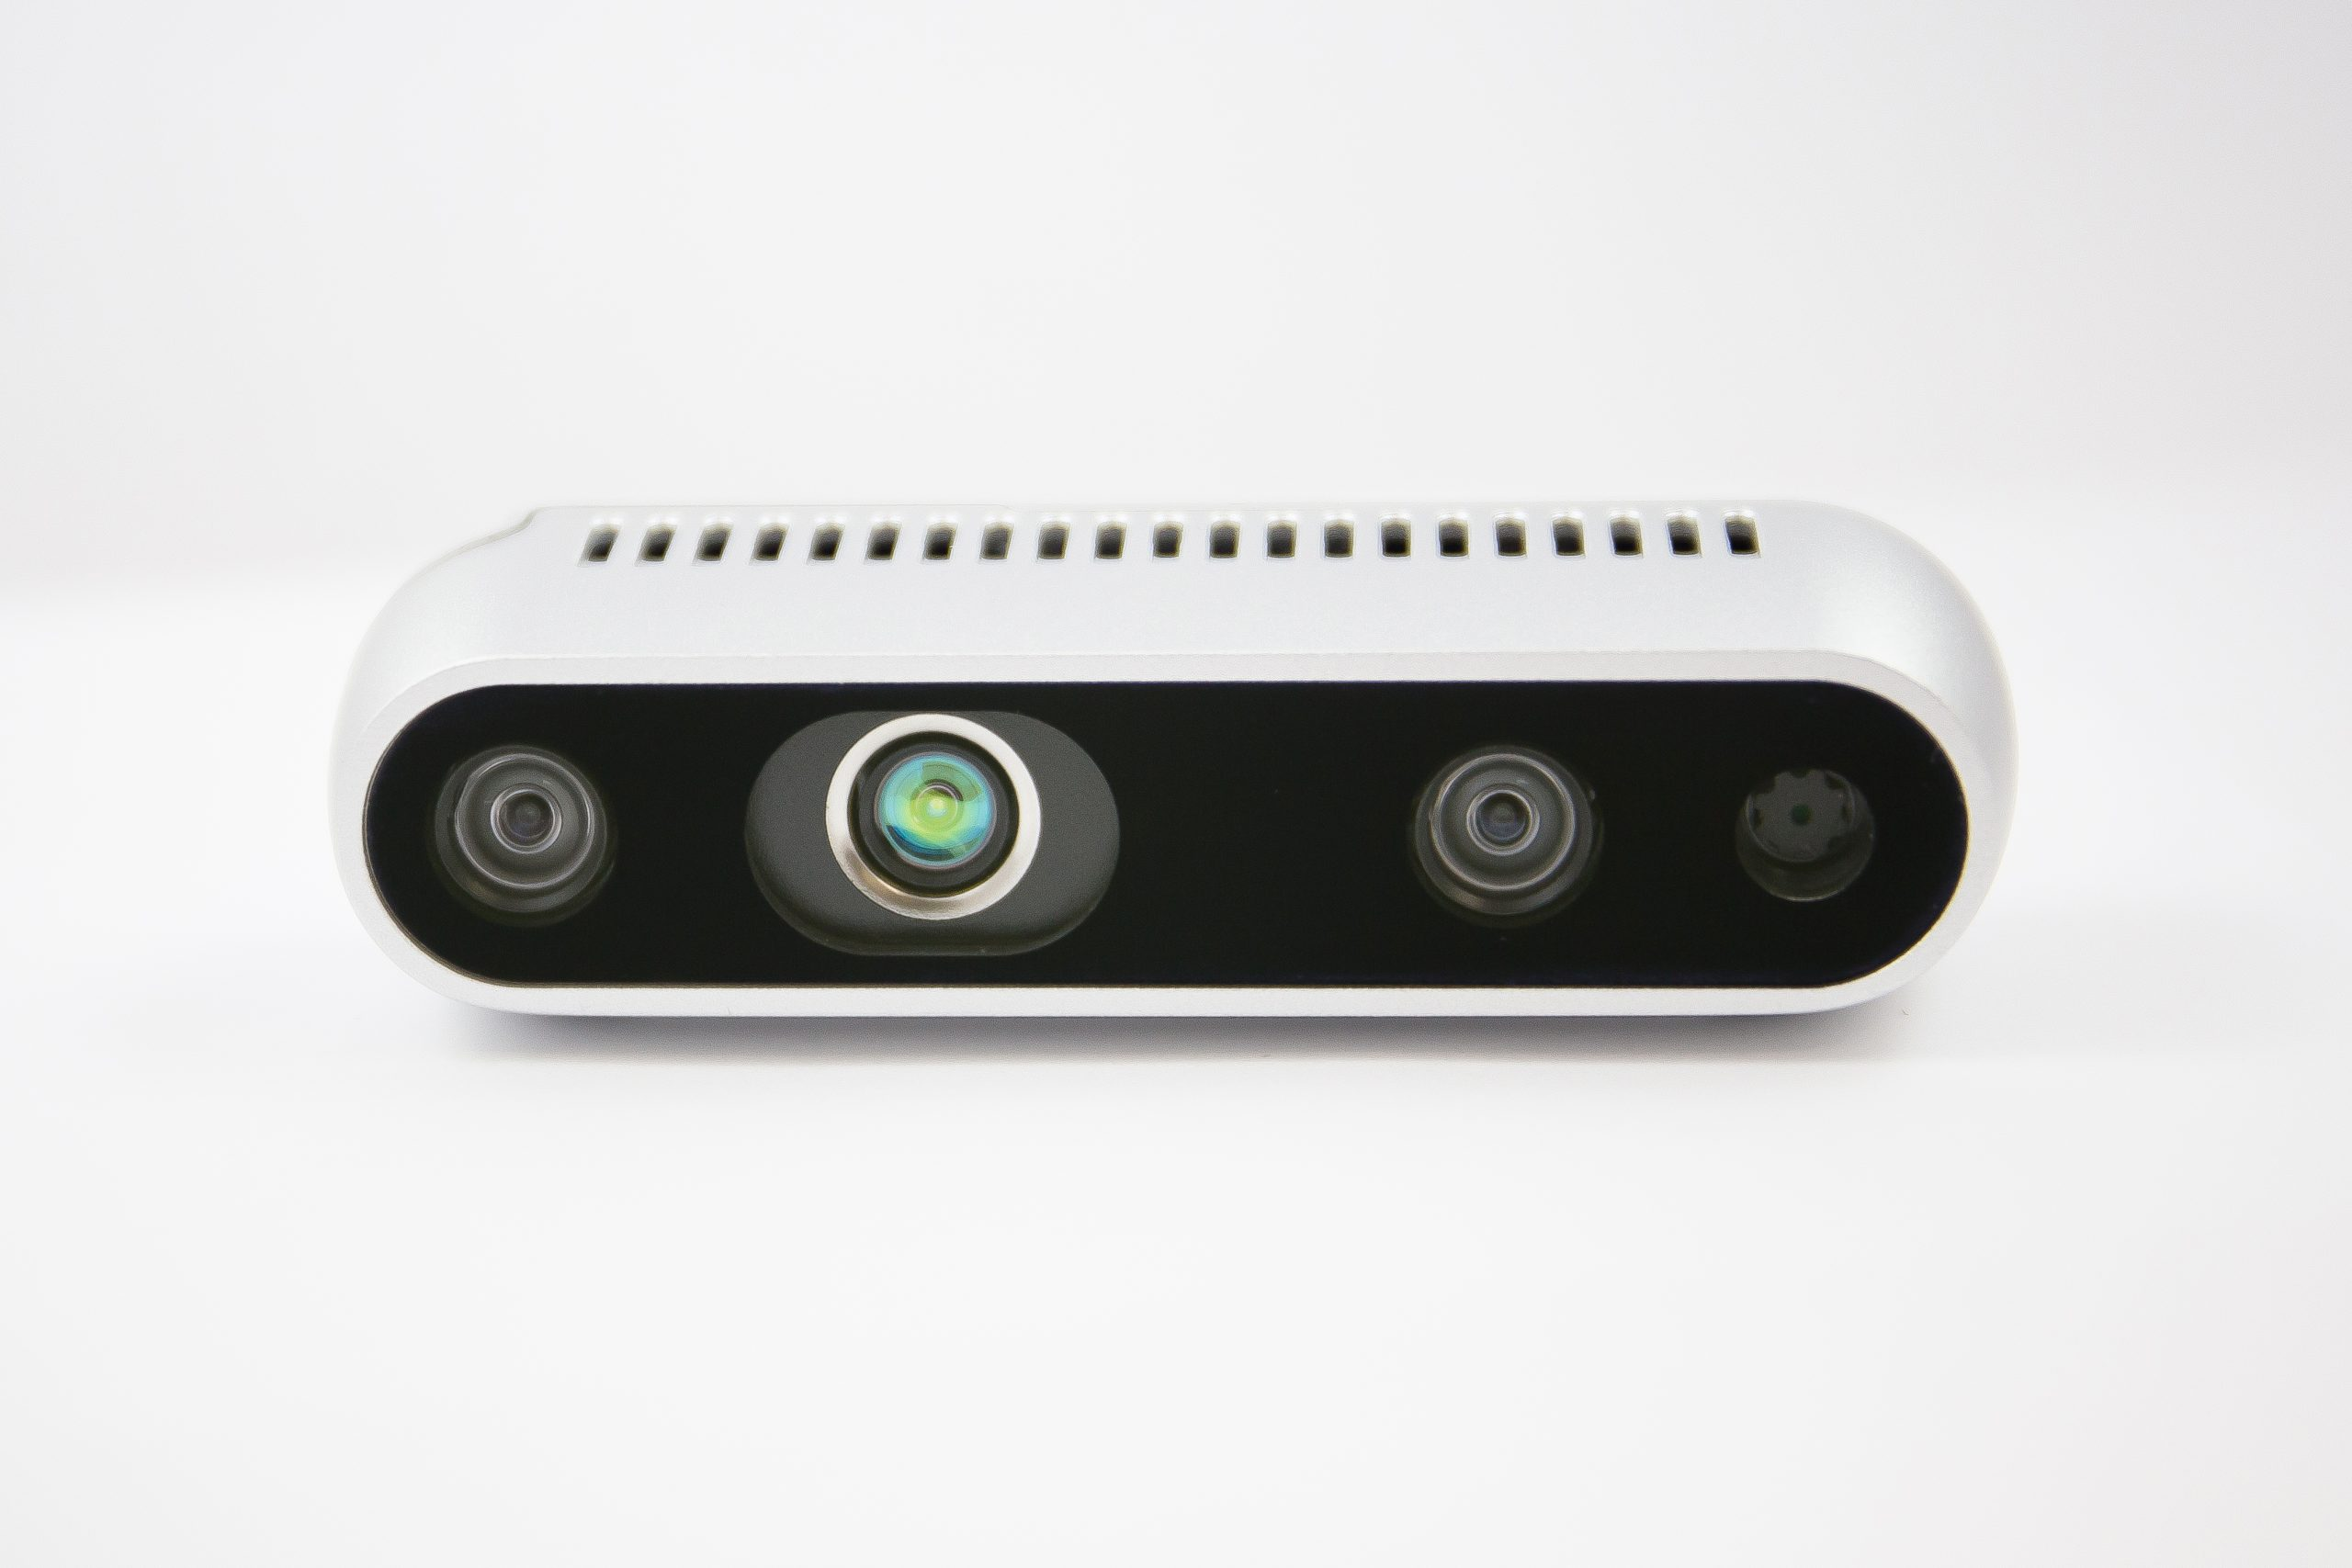
\includegraphics[width=0.5\textwidth]{images/TOF-IR.jpg}  % Adjust the path and width as necessary
    \captionsetup{labelformat=empty, font=footnotesize}
    \caption{Źródło: https://cell-kom.com/inne/21454-kamera-internetowa-full-hd-b16-1080p-5900217390350.html}
    \label{fig:mono}  % Optional: use to refer to this image later in the text
\end{figure}

Time-of-Flight (ToF) to technologia, która służy do mierzenia odległości za pomocą światła, wysyłając impuls świetlny (zwykle w postaci podczerwieni) i rejestrując czas, jaki upływa, zanim światło odbije się od obiektu i wróci do czujnika. Dzięki temu możliwe jest uzyskanie dokładnych pomiarów odległości w czasie rzeczywistym.

\begin{minipage}[t]{0.45\textwidth}
\textbf{Zalety:}
\begin{itemize}
  \item Precyzyjne pomiary – ToF pozwala na bardzo dokładne pomiary odległości, nawet w trudnych warunkach, takich jak słabe oświetlenie.

  \item Szybkość – Technologie ToF oferują bardzo szybkie pomiary, co jest przydatne w systemach wymagających analizy danych w czasie rzeczywistym, np. w robotyce czy samochodach autonomicznych.

  \item Wielozadaniowość – Dzięki ToF możliwe jest uzyskanie mapy głębi w czasie rzeczywistym, co może być użyteczne w takich dziedzinach jak rozpoznawanie twarzy, zautomatyzowane rozpoznawanie obiektów, monitorowanie przestrzeni 3D itp.

  \item Wydajność przy różnych warunkach oświetleniowych – Technologia działa dobrze zarówno w pełnym słońcu, jak i w ciemności, co czyni ją bardziej wszechstronną w porównaniu do innych metod pomiarów odległości, takich jak lidar czy radar.
\end{itemize}
\end{minipage}
\hfill
\begin{minipage}[t]{0.45\textwidth}
\textbf{Wady:}
\begin{itemize}
  \item Czułość na zakłócenia – ToF może być wrażliwa na różne źródła zakłóceń, takie jak silne światło zewnętrzne, np. słońce, które może wpłynąć na dokładność pomiaru.

  \item Ograniczenia w zasięgu – Chociaż ToF oferuje szybkie pomiary, jego zasięg jest ograniczony, a czujniki mogą mieć problemy w przypadku większych odległości.

  \item Jakość obrazu – W niektórych zastosowaniach, jak np. kamera 3D, ToF może generować dane o niższej jakości w porównaniu do innych technologii, takich jak stereo-vision, szczególnie w warunkach złożonych.

  \item Koszt – Zaawansowane czujniki ToF, zwłaszcza te o dużej rozdzielczości, mogą być dość drogie, co może stanowić barierę w masowym wdrożeniu.
\end{itemize}
\end{minipage}

\subsubsection{Structured Light}

\begin{figure}[h]  % 'h' means "here", it places the figure at the current location in the document
    \centering  % Centers the image
    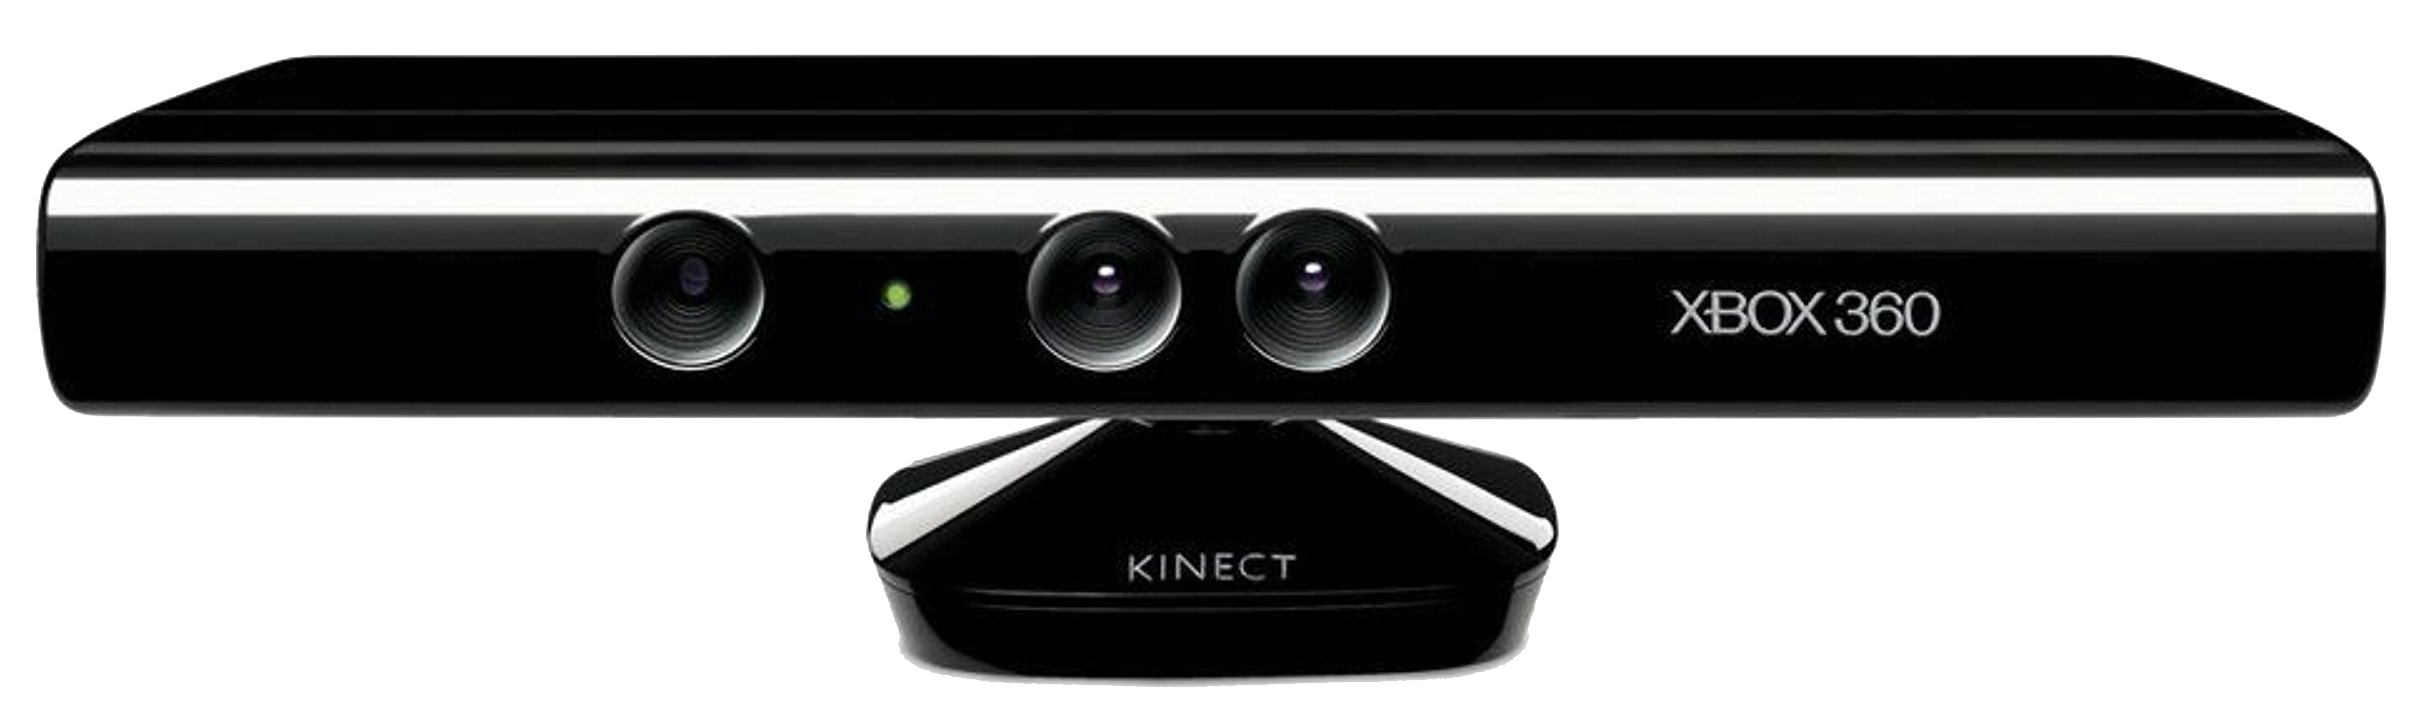
\includegraphics[width=0.5\textwidth]{images/POINTCLOUD.png}  % Adjust the path and width as necessary
    \captionsetup{labelformat=empty, font=footnotesize}
    \caption{Źródło: https://cell-kom.com/inne/21454-kamera-internetowa-full-hd-b16-1080p-5900217390350.html}
    \label{fig:mono}  % Optional: use to refer to this image later in the text
\end{figure}

Structured Light (światło strukturalne) to technologia wykorzystywana do pomiaru głębi i tworzenia map 3D obiektów. Polega na projekcji wzorca świetlnego (np. linii, siatki, wzorów) na powierzchnię obiektu, a następnie analizie deformacji tego wzorca przez czujnik kamery. Na podstawie tych deformacji obliczane są odległości punktów na powierzchni obiektu, co pozwala na stworzenie mapy głębi.

\begin{minipage}[t]{0.45\textwidth}
\textbf{Zalety:}
\begin{itemize}
  \item Wysoka dokładność – Dzięki projekcji specyficznych wzorców świetlnych, ta metoda może zapewnić bardzo dokładne pomiary głębi, szczególnie w porównaniu do innych technologii, takich jak stereo vision.

  \item Szybkość pomiarów – Structured Light pozwala na szybkie tworzenie map 3D, co jest szczególnie przydatne w aplikacjach wymagających analizy w czasie rzeczywistym, jak np. w systemach rozpoznawania twarzy, analizie powierzchni itp.

  \item Dobre działanie w kontrolowanych warunkach – W przypadku dobrze oświetlonych i kontrolowanych warunków (np. w laboratoriach, produkcji), structured light może zapewnić bardzo wysoką jakość obrazu 3D.

  \item Kompatybilność z kamerami RGB – Technologia może być używana w połączeniu z tradycyjnymi kamerami RGB, co pozwala na łatwiejsze połączenie danych o głębi z obrazami kolorowymi.
\end{itemize}
\end{minipage}
\hfill
\begin{minipage}[t]{0.45\textwidth}
\textbf{Wady:}
\begin{itemize}
  \item Wrażliwość na oświetlenie – Structured Light jest wrażliwa na zmieniające się warunki oświetleniowe, zwłaszcza w przypadku silnego, niejednorodnego oświetlenia lub cieni. Może to prowadzić do błędów w pomiarach.

  \item Ograniczona skuteczność na dużych odległościach – Zasięg systemów Structured Light jest zwykle ograniczony do kilku metrów, co sprawia, że nie nadają się one dobrze do pomiarów w dużych przestrzeniach lub na dużych odległościach.

  \item Problemy z teksturami powierzchni – Obiekty o gładkich powierzchniach lub o jednorodnym kolorze mogą sprawiać trudności, ponieważ brak wyraźnych cech do analizy może prowadzić do mniej dokładnych pomiarów.

  \item Złożoność systemu – Aby uzyskać dokładne pomiary, systemy Structured Light wymagają zaawansowanego sprzętu do projekcji wzorców i rejestracji obrazu, co może podnieść koszt urządzenia.
\end{itemize}
\end{minipage}

\subsubsection{LIDAR (Light Detection and Ranging)}

\begin{figure}[h]  % 'h' means "here", it places the figure at the current location in the document
    \centering  % Centers the image
    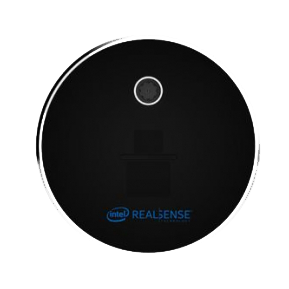
\includegraphics[width=0.5\textwidth]{images/LIDAR.png}  % Adjust the path and width as necessary
    \captionsetup{labelformat=empty, font=footnotesize}
    \caption{Źródło: https://cell-kom.com/inne/21454-kamera-internetowa-full-hd-b16-1080p-5900217390350.html}
    \label{fig:mono}  % Optional: use to refer to this image later in the text
\end{figure}

LIDAR (Light Detection and Ranging) to technologia zdalnego pomiaru odległości, która działa poprzez wysyłanie impulsów laserowych i mierzenie czasu, jaki upływa od ich odbicia od obiektu do powrotu do sensora. Na tej podstawie LIDAR tworzy bardzo dokładne mapy 3D otoczenia.

\begin{minipage}[t]{0.45\textwidth}
\textbf{Zalety:}
\begin{itemize}
  \item Bardzo wysoka dokładność – LIDAR potrafi tworzyć szczegółowe modele 3D otoczenia z dokładnością rzędu centymetrów lub milimetrów.

  \item Długi zasięg – Niektóre systemy LIDAR mogą mierzyć odległości na setki metrów, co sprawia, że są bardzo przydatne w samochodach autonomicznych, dronach i mapowaniu terenu.

  \item Działa w nocy – Ponieważ LIDAR używa własnego źródła światła (lasera), działa niezależnie od oświetlenia zewnętrznego, także w całkowitej ciemności.

  \item Wysoka częstotliwość pomiaru – LIDAR może zbierać dane bardzo szybko, co jest istotne w systemach czasu rzeczywistego, np. podczas jazdy.

  \item Tworzenie map 3D – Idealnie nadaje się do tworzenia chmur punktów i modeli przestrzennych w 3D, np. w kartografii czy inżynierii.
\end{itemize}
\end{minipage}
\hfill
\begin{minipage}[t]{0.45\textwidth}
\textbf{Wady:}
\begin{itemize}
  \item Wysoki koszt – Profesjonalne systemy LIDAR są kosztowne, co ogranicza ich zastosowanie w tanich produktach konsumenckich.

  \item Wrażliwość na warunki atmosferyczne – Deszcz, mgła, śnieg czy kurz mogą zaburzyć pomiary lub obniżyć ich dokładność.

  \item Rozmiar i waga – Choć istnieją miniaturowe wersje, wiele dokładnych systemów LIDAR jest nadal dość duże i ciężkie.

  \item Brak informacji o kolorze/teksturze – LIDAR dostarcza dane o odległości (głębi), ale nie zawiera informacji o kolorze czy wyglądzie powierzchni (w przeciwieństwie do kamer).

\item Ograniczenia w odbiciach od niektórych materiałów – Niektóre powierzchnie, np. czarne lub bardzo błyszczące, mogą słabo odbijać laser, co pogarsza pomiar.
\end{itemize}
\end{minipage}

\subsubsection{Event Cameras (Neuromorphic sensors)}
Capture changes in intensity over time (not full frames).

Can be used for depth estimation when combined with motion.

\section{Natura kamery}

Kamery rejestrują promienie świetlne z naszego otoczenia. Zasadniczo kamera działa jak
nasze oko, odbite promienie światła z naszego otoczenia docierają do naszego oka i są zbierane na siatkówce.
„Kamera otworkowa” jest najprostszym modelem. Jest to dobry uproszczony model do zrozumienia, jak działa kamera. W tym modelu wszystkie promienie światła są zatrzymywane przez powierzchnię. Tylko promienie przechodzące przez otwór są przechwytywane i rzutowane w odwrotnej kolejności na powierzchnię w kamerze. Poniższa ilustracja wyjaśnia tę zasadę

\begin{figure}[h]  % 'h' means "here", it places the figure at the current location in the document
    \centering  % Centers the image
    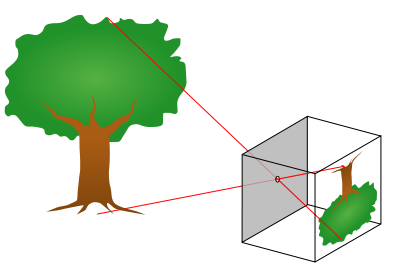
\includegraphics[width=0.5\textwidth]{images/light.png}  % Adjust the path and width as necessary
    \captionsetup{labelformat=empty, font=footnotesize}
    \caption{Źródło: https://funsizephysics.com/use-light-turn-world-upside/}
    \label{fig:rpi}  % Optional: use to refer to this image later in the text
\end{figure}

Zasada ta jest bardzo prosta, ale nie jest to dobry sposób na uchwycenie wystarczającej ilości światła przy szybkiej ekspozycji.
Dlatego soczewki są używane do zbierania promieni światła w jednym miejscu. Problem polega na tym, że taki obiektyw powoduje zniekształcenia.
Istnieją dwa różne rodzaje zniekształceń:
\begin{itemize}
  \item zniekształcenie promieniowe
  \item zniekształcenie styczne
\end{itemize}
Zniekształcenie promieniowe wynika z kształtu samego obiektywu, a zniekształcenie styczne
wynika z geometrii kamery. Obrazy można następnie skorygować za pomocą metod matematycznych.
Proces kalibracji umożliwia stworzenie modelu geometrii kamery i modelu zniekształceń obiektywu.
Modele te tworzą parametry wewnętrzne kamery.

\subsection{Ogniskowa obiektywu}

Względny rozmiar obrazu rzutowanego na powierzchnię w kamerze zależy od ogniskowej.
W modelu otworkowym ogniskowa to odległość między otworem
a obszarem, na który rzutowany jest obraz.
Twierdzenie Talesa daje zatem: $-x = f * (X / Z)$

\begin{itemize}
  \item \textbf{$x$}: obraz obiektu (znak minus wynika z tego, że obraz jest odwrócony)
  \item \textbf{$X$}: rozmiar obiektu
  \item \textbf{$Z$}: odległość od otworu do obiektu
  \item \textbf{$f$}: ogniskowa, odległość od otworu do obrazu
\end{itemize}

\begin{figure}[h]  % 'h' means "here", it places the figure at the current location in the document
    \centering  % Centers the image
    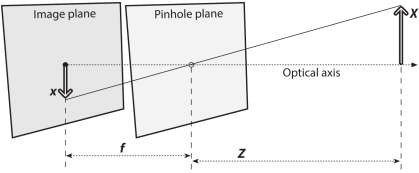
\includegraphics[width=0.5\textwidth]{images/pinhole.png}  % Adjust the path and width as necessary
    \captionsetup{labelformat=empty, font=footnotesize}
    \caption{Źródło: Learning OpenCV 3, O'Reilly, Str. 639}
    \label{fig:rpi}  % Optional: use to refer to this image later in the text
\end{figure}

Ponieważ soczewka nie jest idealnie wyśrodkowana, wprowadzono dwa parametry, $C_x$ i $C_y$, oznaczające odpowiednio poziome i pionowe przemieszczenie soczewki.
Ogniskowa na osiach $X$ i $Y$ są również różne, ponieważ obszar obrazu jest prostokątny. Daje to następujący wzór na położenie obiektu na powierzchni.

\[
x_{\text{screen}} = f_x \left( \frac{X}{Z} \right) + c_x, \quad
y_{\text{screen}} = f_y \left( \frac{Y}{Z} \right) + c_y
\]

Rzutowane punkty świata rzeczywistego na powierzchnię obrazu można zatem modelować w następujący sposób. $M$ jest tutaj macierzą wewnętrzną.

\[
q = MQ, \quad \text{gdzie} \quad
q = \begin{bmatrix} x \\ y \\ w \end{bmatrix}, \quad
M = \begin{bmatrix}
f_x & 0 & c_x \\
0 & f_y & c_y \\
0 & 0 & 1
\end{bmatrix}, \quad
Q = \begin{bmatrix} X \\ Y \\ Z \end{bmatrix}
\]

\subsection{Zniekształcenie obiektywu}

\begin{figure}[h]  % 'h' means "here", it places the figure at the current location in the document
    \centering  % Centers the image
    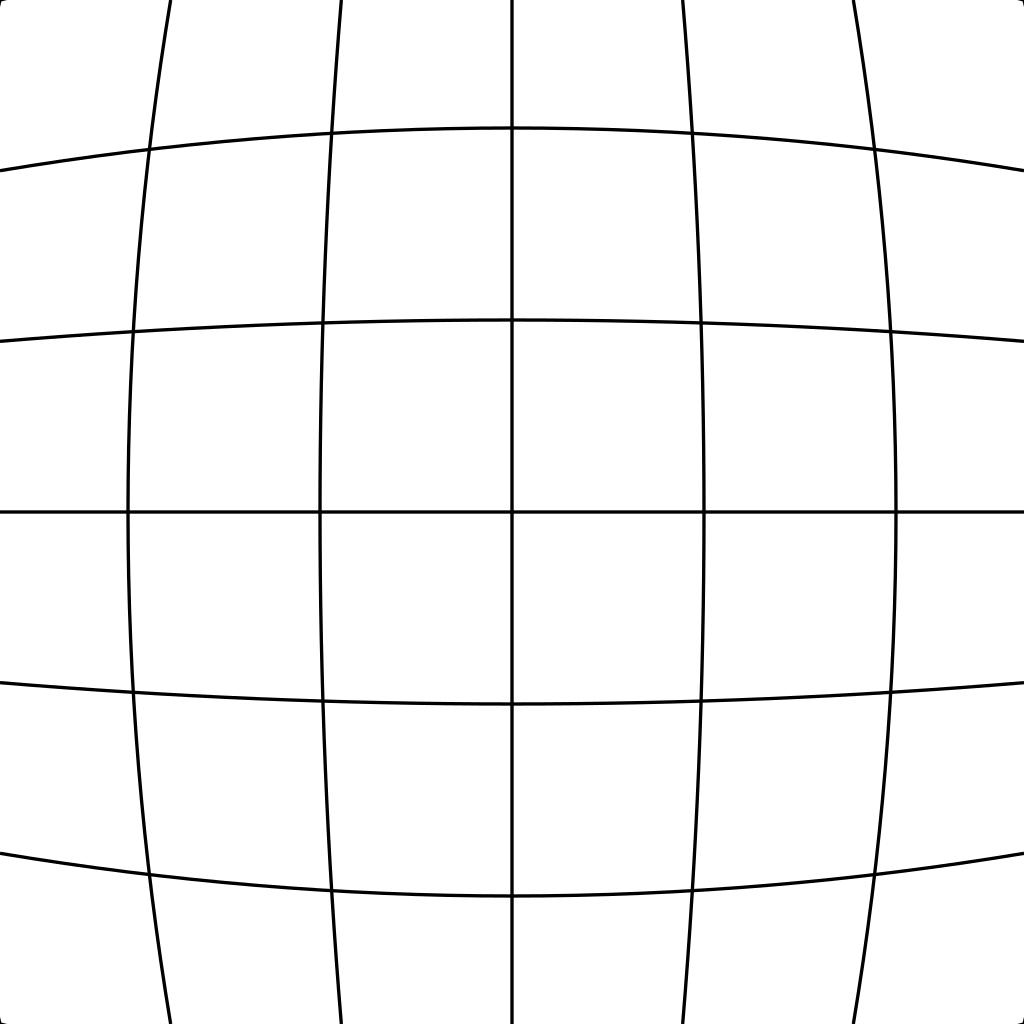
\includegraphics[width=0.3\textwidth]{images/barrel.png}  % Adjust the path and width as necessary
    \captionsetup{labelformat=empty, font=footnotesize}
    \caption{Źródło: Wikipedia}
    \label{fig:rpi}  % Optional: use to refer to this image later in the text
\end{figure}

Teoretycznie możliwe jest zbudowanie obiektywu, który nie powoduje zniekształceń za pomocą soczewki parabolicznej.
W praktyce jednak znacznie łatwiej jest stworzyć soczewkę sferyczną niż paraboliczną.
Jak wspomniano wcześniej, istnieją dwa rodzaje zniekształceń. Zniekształcenie
promieniowe, które wynikają z kształtu obiektywu i zniekształcenia styczne spowodowane procesem montażu kamery.

W centrum optycznym nie ma zniekształceń promieniowych, a przy zbliżaniu się do krawędzi stają się one coraz większe, gdy zbliżamy się do krawędzi. W praktyce zniekształcenie to pozostaje niewielkie, wystarczy wykonać rozwinięcie Taylora do trzeciego członu.
Daje to następujący wzór.

\begin{align*}
x_{\text{corrected}} &= x \left(1 + k_1 r^2 + k_2 r^4 + k_3 r^6 \right) \\
y_{\text{corrected}} &= y \left(1 + k_1 r^2 + k_2 r^4 + k_3 r^6 \right)
\end{align*}

$x$ i $y$ to współrzędne oryginalnego punktu na obszarze obrazu, które są używane do obliczenia pozycji skorygowanego punktu.
skorygowanego punktu.
Występuje również zniekształcenie styczne, ponieważ obiektyw nie jest idealnie
idealnie równoległa do powierzchni obrazu. Aby to skorygować
wprowadzane są dwa dodatkowe parametry, $p_1$ i $p_2$.

\begin{align*}
x_{\text{corrected}} &= x + \left[2p_1 y + p_2 (r^2 + 2x^2)\right] \\
y_{\text{corrected}} &= y + \left[p_1 (r^2 + 2y^2) + 2p_2 x\right]
\end{align*}


\section{Obrazowanie stereoskopowe}

Stereo Vision umożliwia rozpoznawanie głębi na obrazie, wykonywanie pomiarów na obrazie
i przeprowadzanie lokalizacji 3D. Między innymi należy znaleźć punkty, które pasują do siebie między dwiema kamerami. Można to następnie wykorzystać do odległość między kamerą a punktem. Wykorzystywana jest geometria systemu w celu uproszczenia obliczeń.

Te cztery kroki są wykonywane podczas obrazowania stereo:

\begin{enumerate}
  \item usuwanie zniekształceń promieniowych i stycznych za pomocą obliczeń matematycznych
obliczenia. W ten sposób powstają obrazy bez deformacji.
  \item rektyfikacja kąta i odległości obrazów. Na tym etapie oba obrazy są
obrazy współpłaszczyznowe na osi $Y$, co ułatwia wyszukiwanie korespondencji.
łatwiejsze i wystarczy szukać tylko na jednej osi (osi $X$).
  \item znajdź tę samą cechę na prawym i lewym obrazie. Daje to mapę dysproporcji pokazującą różnice między obrazami na osi $X$.
  \item Ostatnim krokiem jest triangulacja. Mapa rozbieżności jest przekształcana w odległości za pomocą triangulacji.
\end{enumerate}

\subsection{Triangulacja}

\begin{figure}[h]  % 'h' means "here", it places the figure at the current location in the document
    \centering  % Centers the image
    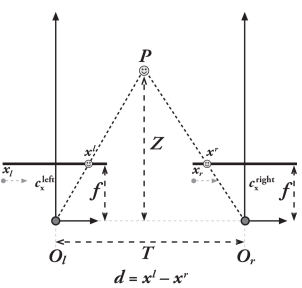
\includegraphics[width=0.5\textwidth]{images/triangulation.png}  % Adjust the path and width as necessary
    \captionsetup{labelformat=empty, font=footnotesize}
    \caption{Źródło: Learning OpenCV 3, O'Reilly, Str. 705}
    \label{fig:rpi}  % Optional: use to refer to this image later in the text
\end{figure}

W ostatnim kroku, triangulacji, zakłada się, że oba obrazy projekcji są współpłaszczyznowe i że poziomy rząd pikseli lewego obrazu jest wyrównany z odpowiadającym mu obrazem prawego.

Poniższy obraz można teraz skonstruować przy użyciu poprzednich hipotez.

Punkt $P$ leży w środowisku i jest pokazany na
lewym i prawym obrazie na $P_l$ i $P_r$, z odpowiadającymi im współrzędnymi
odpowiadającymi współrzędnymi $X_l$ i $X_r$. To
pozwala nam wprowadzić nową wielkość
$d = X_l - X_r$. Można zauważyć, że im dalej punkt
punkt $P$, tym mniejsza staje się wielkość $d$. Dysproporcja
jest zatem odwrotnie proporcjonalna do odległości.
odległości.\\
Do obliczenia odległości można użyć następującego wzoru
można obliczyć: \[Z=f*T/(xl-xr)\]

Można zauważyć, że istnieje nieliniowa zależność między rozbieżnością a odległością.
Jeśli rozbieżność jest bliska 0, małe różnice w rozbieżności prowadzą do dużych różnic w odległości.
Zjawisko to ulega odwróceniu, gdy rozbieżność jest duża. Małe różnice dysproporcji nie prowadzą do dużych różnic odległości. Na tej podstawie można wywnioskować, że stereowizja ma wysoką rozdzielczość głębi, tylko dla obiektów znajdujących się blisko kamery.

Metoda ta działa jednak tylko wtedy, gdy konfiguracja kamery stereo jest idealna. W
rzeczywistości tak nie jest. Właśnie dlatego lewy i prawy obraz są
matematycznie wyrównane równolegle. Oczywiście kamery muszą być fizycznie ustawione równolegle.
Zanim zostanie wyjaśniona metoda matematycznego wyrównywania obrazów, trzeba najpierw zrozumieć geometrię epipolarną.

\subsection{Geometria epipolarna}

\begin{figure}[h]  % 'h' means "here", it places the figure at the current location in the document
    \centering  % Centers the image
    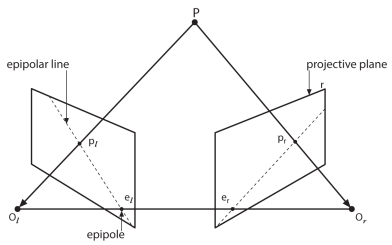
\includegraphics[width=0.7\textwidth]{images/epipolar.png}  % Adjust the path and width as necessary
    \captionsetup{labelformat=empty, font=footnotesize}
    \caption{Źródło: Learning OpenCV 3, O'Reilly, Str. 709}
    \label{fig:rpi}  % Optional: use to refer to this image later in the text
\end{figure}

Powyższy obrazek przedstawia model niedoskonałej kamery stereo składającej się z dwóch modeli kamer otworkowych.
Przecięcie linii środków projekcji ($O_l$, $O_r$) z płaszczyznami projekcji tworzone są punkty epipolarne $e_l$ i $e_r$. Linie ($p_l$, $e_l$) i ($p_r$, $e_r$) są nazywane liniami epipolarnymi. Obrazem wszystkich możliwych punktów punktu
na płaszczyźnie rzutowania jest linia epipolarna, która leży na drugiej płaszczyźnie obrazu i
przechodzi przez punkt epipolarny i szukany punkt. Umożliwia to ograniczenie wyszukiwania punktu na jednym wymiarze zamiast na całej płaszczyźnie.\\
Można zatem podsumować następujące punkty:

\begin{itemize}
  \item Każdy punkt 3D w widoku kamery jest zawarty w planie epipolarnym
  \item Element w jednej płaszczyźnie musi znajdować się na odpowiednich liniach epipolarnych drugiej płaszczyzny (warunek epipolarny).
drugiej płaszczyzny (warunek epipolarny)
  \item Dwuwymiarowe wyszukiwanie odpowiadającego elementu jest konwertowane na
jednowymiarowe, jeśli znana jest geometria epipolarna.
  \item Kolejność punktów jest zachowana, tzn. dwa punkty $A$ i $B$ są w tej samej kolejności na liniach epipolarnych płaszczyzny.

\end{itemize}

ta sama kolejność na liniach epipolarnych jednej płaszczyzny, co na liniach epipolarnych drugiej płaszczyzny.

\subsection{Macierze podstawowe i fundamentalne}

Aby zrozumieć, w jaki sposób obliczane są linie epipolarne, musimy najpierw wyjaśnić macierze podstawowe
i macierze fundamentalne (odpowiadające macierzom $E$ i $F$).
Macierz podstawowa $E$ zawiera informacje o tym, jak fizycznie rozmieszczone są obie kamery.
Opisuje ona lokalizację drugiej kamery względem pierwszej za pomocą parametrów translacji i rotacji.
Parametrów tych nie można odczytać bezpośrednio w macierzy, ponieważ jest ona używana do planowania projektu. W sekcji Kalibracja stereo wyjaśnone będzie, jak obliczyć $R$ i $T$ (macierz rotacji i wektor translacji).
Macierz $F$ zawiera informacje z podstawowej macierzy $E$, fizyczny układ kamer i informacje o wewnętrznych parametrach kamer.
Relacja między rzutowanym punktem na lewym obrazie $p_l$ i rzutowanym punktem na prawym obrazie $p_r$ jest zdefiniowana następująco:

\[prTEpl=0\]
Można by pomyśleć, że ta formuła w pełni opisuje związek między lewym i prawym punktem.
prawym punktem. Należy jednak zauważyć, że macierz 3x3 $E$ jest rzędu
jest rangi 2. Oznacza to, że wzór ten jest równaniem prostej.
Aby w pełni zdefiniować relację między punktami, parametry wewnętrzne.
parametry wewnętrzne.
Pamiętamy, że $q = Mp$, z macierzą wewnętrzną $M$.
Podstawienie do poprzedniego równania daje wynik:
\[qrT(Ml-1)TEMl-1ql=0\]
Podstawienie:\\
\[F=(Ml-1)TEMl-1\]
W ten sposób otrzymujemy\\
\[qrTFql=0\]

\subsection{Macierz obrotu i wektor przesunięcia}

Teraz, gdy zostałą wyjaśniona macierz podstawową $E$ i macierz podstawową $F$, trzeba zobaczyć, jak obliczyć macierz obrotu i wektor translacji.
Zdefiniujemy następujące oznaczenia:

\begin{itemize}
  \item $P_l$ i $P_r$ definiują pozycje punktu w układzie współrzędnych odpowiednio lewej i prawej kamery.
  \item $R_l$ i $T_l$ (lub $R_r$ i $T_r$) definiują obrót i translację z kamery
do punktu w otoczeniu dla lewej (lub prawej) kamery.
  \item $R$ i $T$ to obrót i translacja układu współrzędnych prawej kamery w układzie współrzędnych lewej kamery.
\end{itemize}

Daje to następujące wyniki
\[
\begin{array}{cc}
P_l = R_l P + T_l & \quad P_r = R_r P + T_r
\end{array}
\]
Mamy również:
\[Pl=RT(Pr-T)\]
Z tych trzech równań ostateczny wynik to
\[
\begin{array}{cc}
R = R_r R_l^T & \quad T = T_r - R T_l
\end{array}
\]




\subsection{Rektyfikacja stereo}

Dotychczas zajmowaliśmy się tematem „kalibracji stereo”. Chodziło o
opis geometrycznego rozmieszczenia obu kamer. Zadaniem
rektyfikacji jest rzutowanie dwóch obrazów tak, aby leżały dokładnie w tej samej płaszczyźnie i precyzyjne wyrównanie rzędów pikseli tak, aby linie epipolarne stały się poziome w celu zapewnienia zgodności punktu na dwóch obrazach.
aby znaleźć zgodność punktu na dwóch obrazach w sposób bardziej losowy.
W wyniku procesu wyrównywania obu obrazów uzyskuje się 8 wyrażeń, po 4 dla każdej kamery:

\begin{itemize}
  \item wektor zniekształceń
  \item macierz rotacji Rrect, która musi zostać zastosowana do obrazu
  \item wyprostowana macierz kamery Mrect
  \item nierektyfikowana macierz kamery $M$
\end{itemize}

OpenCV pozwala nam obliczyć te warunki za pomocą dwóch algorytmów: algorytmu Hartley'a
i algorytmu Bouguet'a.

\subsubsection{Algorytm Hartley'a}

Algorytm Hartleya wyszukuje te same punkty na obu obrazach. Próbuje on
stara się zminimalizować rozbieżności i znaleźć homografie, które ustawiają epipole w nieskończoności.
nieskończoność. Dzięki tej metodzie nie jest więc konieczne obliczanie parametrów wewnętrznych dla każdej kamery.
dla każdej kamery.
Zaletą tej metody jest to, że kalibracja jest możliwa tylko dzięki obserwacji punktów w scenie.
punktów na scenie. Główną wadą jest jednak brak skalowania obrazu
Masz tylko informacje o względnej odległości. Nie można dokładnie zmierzyć
jak daleko obiekt znajduje się od kamer.

\subsubsection{Algorytm Bouguet'a}

Algorytm Bougueta wykorzystuje obliczoną macierz obrotu i wektor translacji
aby obrócić obie rzutowane płaszczyzny o pół obrotu, tak aby znalazły się w tej samej płaszczyźnie.
tej samej płaszczyźnie. Sprawia to, że główne promienie są równoległe, a płaszczyzny współpłaszczyznowe.
ale nie są jeszcze wyrównane w rzędach. Zostanie to zrobione później.
W projekcie wykorzystaliśmy algorytm Bougueta.

\chapter{Rozdział badawczy}

\section{Opis projektu}

\begin{figure}[h]  % 'h' means "here", it places the figure at the current location in the document
    \centering  % Centers the image
    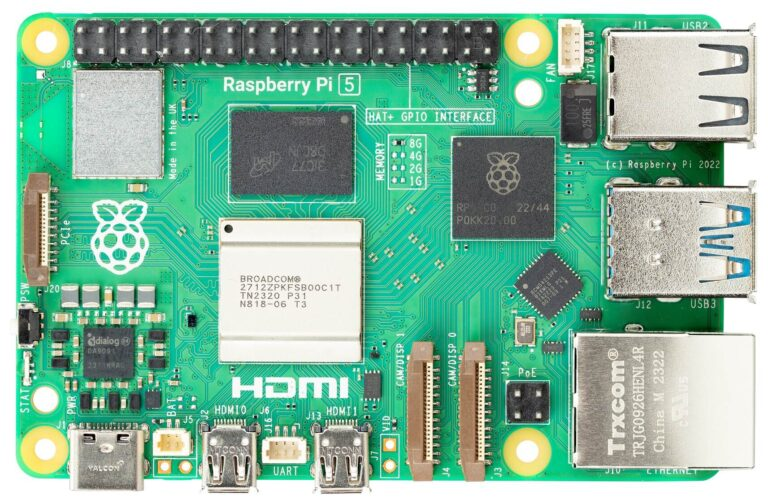
\includegraphics[width=0.5\textwidth]{images/RPI.jpg}  % Adjust the path and width as necessary
    \captionsetup{labelformat=empty, font=footnotesize}
    \caption{Źródło: https://www.hackatronic.com/wp-content/uploads/2023/11/Raspberry-5-pi-.jpg}
    \label{fig:rpi}  % Optional: use to refer to this image later in the text
\end{figure}

\begin{figure}[h]  % 'h' means "here", it places the figure at the current location in the document
    \centering  % Centers the image
    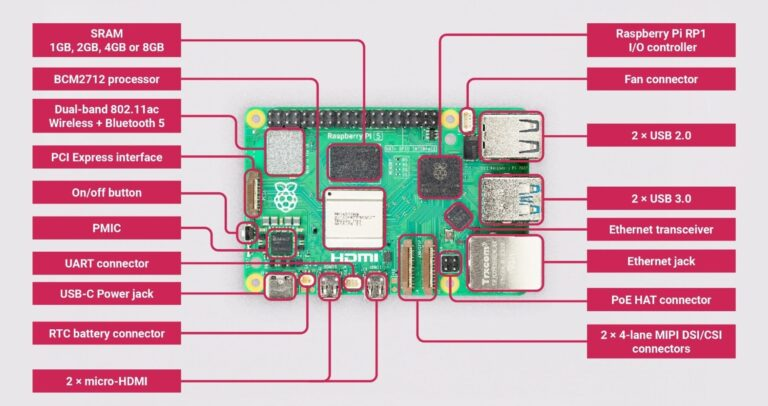
\includegraphics[width=0.7\textwidth]{images/RPI-SPEC.jpg}  % Adjust the path and width as necessary
    \captionsetup{labelformat=empty, font=footnotesize}
    \caption{Źródło: https://www.hackatronic.com/wp-content/uploads/2024/03/Raspberry-Pi-5-Pinout--1210x642.jpg}
    \label{fig:rpi-spec}  % Optional: use to refer to this image later in the text
\end{figure}

\begin{figure}[h]  % 'h' means "here", it places the figure at the current location in the document
    \centering  % Centers the image
    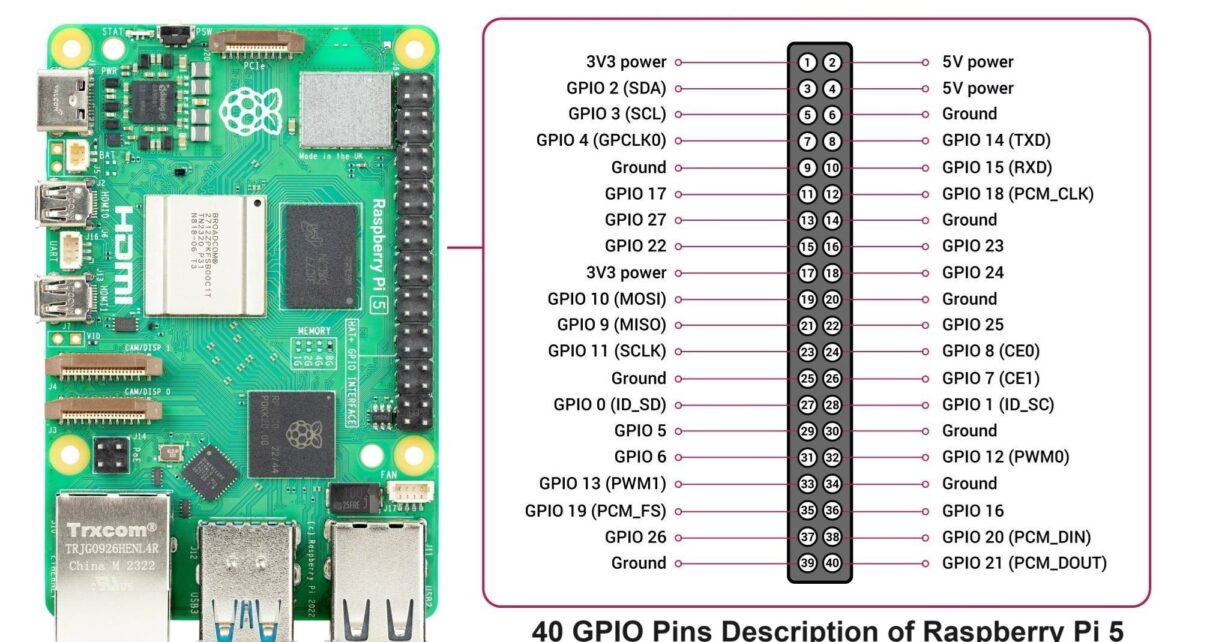
\includegraphics[width=0.5\textwidth]{images/RPI-PIN.jpg}  % Adjust the path and width as necessary
    \captionsetup{labelformat=empty, font=footnotesize}
    \caption{Źródło: https://www.hackatronic.com/wp-content/uploads/2024/03/Raspberry-Pi-5-Pinout--1210x642.jpg}
    \label{fig:rpi-gpio}  % Optional: use to refer to this image later in the text
\end{figure}

\begin{figure}[h]  % 'h' means "here", it places the figure at the current location in the document
    \centering  % Centers the image
    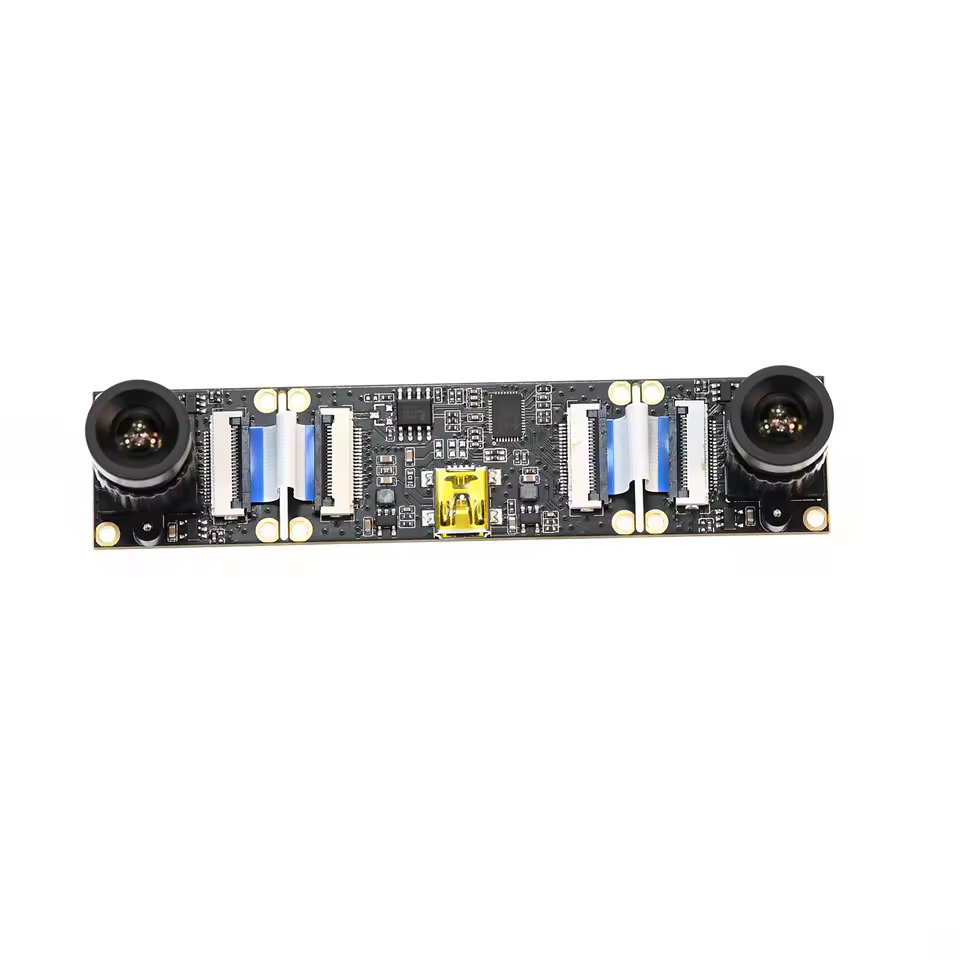
\includegraphics[width=0.5\textwidth]{images/MAINSTEREO.png}  % Adjust the path and width as necessary
    \captionsetup{labelformat=empty, font=footnotesize}
    \caption{Źródło: https://pl.aliexpress.com/i/1005006618001887.html}
    \label{fig:mono}  % Optional: use to refer to this image later in the text
\end{figure}

\section{Funkcjonalność programu do obrazowania stereo}

Jak już wspomniano, program jest kodowany w Pythonie i wykorzystywana jest biblioteka OpenCV.
jest używana. Zdecydowaliśmy się na język Python i bibliotekę OpenCV, ponieważ
mieliśmy już z nimi doświadczenie i ponieważ istnieje wiele dokumentacji na ich temat. Innym
argumentem za tą decyzją jest to, że chcieliśmy pracować tylko z bibliotekami „open source”.
biblioteki.
Na potrzeby tego projektu opracowano dwa programy w języku Python.
Pierwszy z nich, „Take-images-for-calibration.py”, służy do robienia dobrych zdjęć, które są później wykorzystywane do kalibracji obu kamer.
Później są one wykorzystywane do kalibracji obu kamer (kalibracja zniekształceń i kalibracja stereo).
kalibracja.
Drugi program, a tym samym główny program „Main-Stereo-Vision-Prog.py” jest używany do obrazowania stereo.
jest używany do obrazowania stereo. W tym programie kalibrujemy kamery za pomocą wykonanych zdjęć, generujemy mapę dysproporcji i dzięki doświadczalnemu równaniu
równania, które zostało znalezione eksperymentalnie, możemy zmierzyć odległość dla każdego piksela.
pomiar. Na końcu używany jest filtr WLS, aby lepiej rozpoznawać krawędzie obiektów.
rozpoznać krawędzie obiektów.

\subsection{Wykorzystane pakiety}

Do programu zaimportowano następujące pakiety:
- Wersja OpenCV.3.2.0 z opencv-contrib (zawiera funkcje stereo) jako.
„cv2” w Pythonie, zawiera:
o bibliotekę do przetwarzania obrazów
o funkcje do stereowizji
- Numpy.1.12.
o Używany do operacji na macierzach (obrazy składają się z macierzy)
- Skoroszyt z openpyxl
o Pakiet umożliwiający zapisywanie danych w pliku Excel
- „normalizacja” biblioteki sklearn 0.18.1
o sklearn umożliwia uczenie maszynowe, ale w tym projekcie używany jest
tylko filtr WLS

\subsection{Główna pętla}

Aby pracować z kamerami, należy je najpierw aktywować. Funkcja
cv2.VideoCapture() aktywuje obie kamery poprzez wprowadzenie numeru portu każdej z nich.
kamery (w programie tworzone są dwa obiekty korzystające z metod klasy cv2.VideoCapture()).
klasy cv2.VideoCapture()).

Aby uzyskać obraz z kamer, używana jest metoda cv2.VideoCapture().read()
Wyjściem jest obraz sceny, którą kamera ogląda w momencie wywołania tej funkcji.
funkcja jest wywoływana. Aby uzyskać obraz wideo, należy wywołać tę metodę
w nieskończonej pętli. Aby być bardziej wydajnym, zaleca się
aby przekonwertować obrazy BGR na obrazy w odcieniach szarości, odbywa się to za pomocą funkcji cv2.cvtColor()
funkcja.

Aby wyświetlić wideo na komputerze, używana jest funkcja cv2.imshow().
aby otworzyć okno, w którym można wyświetlić wideo.

Przerwanie służy do wyjścia z nieskończonej pętli. Staje się ona aktywna
za każdym razem, gdy użytkownik naciśnie spację. Rozpoznanie, że klawisz został naciśnięty
jest rozpoznawane dzięki funkcji cv2.waitKey().
Wreszcie, dwie używane kamery muszą zostać dezaktywowane za pomocą metody
cv2.VideoCapture().release(), a otwarte okna są niszczone za pomocą funkcji
cv2.destroyAllWindows().

\subsection{Funkcjonalność programu „Take-images-for-calibration.py”}

Po uruchomieniu tego programu obie kamery stają się aktywne i otwierane są dwa okna.
aby użytkownik mógł zobaczyć, gdzie na obrazach znajduje się szachownica.


\subsubsection{Kalibracja za pomocą OpenCV}

Biblioteka OpenCV pozwala nam obliczyć parametry wewnętrzne za pomocą określonych funkcji.
Proces ten nazywany jest kalibracją. Jest to możliwe dzięki różnym
widoków szachownicy.

Program do robienia zdjęć do późniejszej kalibracji nosi nazwę
„Take-images-for-calibration.py”.
Jeśli rogi szachownicy zostaną rozpoznane na obu kamerach, otworzą się dwa okna z rozpoznanym obrazem dla każdej kamery.
z rozpoznanym obrazem dla każdej kamery. Obrazy są następnie zapisywane lub usuwane
zapisywane lub usuwane. Można rozpoznać dobre obrazy, na których narożniki
są bardzo wyraźnie rozpoznawalne. Obrazy te są później używane do kalibracji w głównym programie
programie „Main-Stereo-Vision-Prog.py”. OpenCV zaleca posiadanie co najmniej 10
obrazów dla każdej kamery, aby uzyskać dobrą kalibrację. My uzyskaliśmy dobre wyniki przy 50
obrazów dla każdej kamery.
Aby skalibrować kamery, kod Pythona wyszukuje narożniki szachownicy na każdym
obrazie dla każdej kamery przy użyciu funkcji OpenCV: cv2.findChesssboardCorners

Pozycja narożników dla każdego obrazu jest następnie zapisywana w wektorze obrazu, a punkty obiektu dla sceny 3D są zapisywane w innym wektorze.
dla sceny 3D są zapisywane w innym wektorze. Następnie należy użyć
następnie użyć tych Imgpoints i Objpoints w funkcji cv2.calibeCamera(), której wynikiem jest
macierz kamery, współczynniki zniekształceń, wektory obrotu i translacji
są zwracane.

Funkcja cv2.getOptimalNewCameraMatrix() umożliwia nam uzyskanie dokładnych macierzy kamer.
które później wykorzystamy w funkcji cv2.stereoRectify().

Po kalibracji za pomocą OpenCV otrzymujemy następującą macierz M dla naszej kamery:

Matryca M bez rektyfikacji (prawa kamera):

Matrix Mrekt Rectified (prawa kamera):

Matryca M bez rektyfikacji (lewa kamera):

Matryca M wyprostowana (lewa kamera):

\subsubsection{Wektory kalibracyjne}

Funkcja cv2.findChessboardCorners() wyszuka określoną liczbę narożników szachownicy
i wygenerowane zostaną następujące wektory:

\begin{itemize}
  \item imgpointsR: zawiera współrzędne narożników na prawym obrazie (w przestrzeni obrazu)
  \item imgpointsL: zawiera współrzędne narożników na lewym obrazie (w przestrzeni obrazu)
  \item objpoints: zawiera współrzędne narożników w przestrzeni obiektu.
\end{itemize}

Precyzja współrzędnych znalezionych narożników jest zwiększana za pomocą funkcji
cv2.cornerSubPix().

\subsubsection{Pozyskiwanie obrazów do kalibracji}
\subsection{Funkcjonalność programu „Main-Stereo-Vision-Prog.py”}
\subsubsection{Kalibracja zniekształceń}
\subsubsection{Kalibracja kamery stereo}
\subsubsection{Obliczanie mapy rozbieżności}
\subsubsection{Zastosowanie filtra WLS (ważonych najmniejszych kwadratów)}
\subsubsection{Pomiar odległości}
\subsubsection{Możliwe ulepszenia}

\chapter{Zakończenie}

\begin{thebibliography}{7}
\addcontentsline{toc}{chapter}{Bibliografia}

\bibitem{opencv}
OpenCV, 
\textit{https://opencv.org}.

\bibitem{Lambert} 
Stereo and Disparity, John Lambert,  
\textit{https://johnwlambert.github.io/stereo/}.

\bibitem{rao} 
Stereo and 3D Vision, Rajesh Rao, 
\textit{https://courses.cs.washington.edu/courses/cse455/09wi/Lects/lect16.pdf}.

\bibitem{reilly} 
Learning OpenCV 3, O'Reilly. 

\end{thebibliography}
\end{document}
